\subsection{Lớp mật mã — EC-Schnorr Blind Multisignature}

\subsubsection{Lý do lựa chọn EC-Schnorr trên đường cong secp256k1}

Toàn bộ lớp mật mã của hệ thống được xây dựng quanh lược đồ chữ ký mù tập thể EC-Schnorr trên đường cong elliptic \pkg{secp256k1}. Đây là kết quả cân nhắc giữa hai tiêu chí thực tế: tính \textit{linearity} của Schnorr cho phép tổng hợp chữ ký không tương tác, đồng thời kích thước scalar và point trên \pkg{secp256k1} nhỏ hơn nhiều so với khóa DSA/RSA cùng mức an toàn. Bảng~\ref{tab:so-sanh-schnorr} đối chiếu một số tiêu chí then chốt giữa hai họ lược đồ.

\begin{table}[H]
\centering
\caption{So sánh tiêu chí kỹ thuật giữa DSA/RSA và EC-Schnorr trên secp256k1}
\label{tab:so-sanh-schnorr}
\begin{tabularx}{\textwidth}{|L{0.35}|L{0.3}|L{0.45}|}
\hline
\textbf{Tiêu chí} & \textbf{DSA/RSA 2048-bit} & \textbf{EC-Schnorr secp256k1} \\
\hline
Mức bảo mật & xấp xỉ 112-bit & xấp xỉ 128-bit \\
\hline
Kích thước scalar & 256 byte & 32 byte (nhỏ hơn 8 lần) \\
\hline
Kích thước point & không áp dụng & 33 byte (dạng nén) \\
\hline
Tốc độ nhân vô hướng & cơ sở & nhanh hơn từ 5 đến 25 lần \\
\hline
Tính tổng hợp (\textit{linearity}) & không hỗ trợ & có — $s = \sum s_i \bmod n$ \\
\hline
Hỗ trợ tạo chữ ký mù & phức tạp & tự nhiên qua các hệ số làm mù \\
\hline
\end{tabularx}
\end{table}

Tính \textit{linearity} là yếu tố mang tính quyết định trong kiến trúc nhiều nút ký: ba nút ký độc lập, mỗi nút sinh chữ ký phần (\textit{partial signature}) của riêng mình, sau đó bộ điều phối chỉ cần cộng dồn các giá trị scalar — không cần một vòng giao tiếp bổ sung và không tạo ra ràng buộc lệ thuộc lẫn nhau giữa các nút.

\subsubsection{Giao thức ký mù tập thể}

Tham số hệ thống được cố định cho toàn bộ vòng đời ứng dụng:

\begin{verbatim}
Curve:  secp256k1
n:      bậc của nhóm (256-bit)
G:      điểm sinh chuẩn
SCALAR_BYTES = 32,  POINT_BYTES = 33 (compressed)
\end{verbatim}

Giao thức được chia thành sáu pha hoạt động tuần tự, trải dài trên ba thực thể là cử tri (trình duyệt), bộ điều phối (\textit{Coordinator}) và ba nút ký (\textit{Signing Nodes}):

\begin{itemize}
    \item \textbf{Pha 0 -- Sinh khóa:} mỗi nút ký $i$ sinh khóa bí mật $d_i \in [1, n-1]$ và công bố khóa công khai phần $P_i = d_i \cdot G$. Bộ điều phối tính khóa công khai tập thể $P_{agg} = P_1 + P_2 + P_3$.

    \item \textbf{Pha 1 -- Cam kết:} khi bắt đầu phiên, mỗi nút ký sinh nonce ngẫu nhiên $k_i$ và điểm cam kết $R_i = k_i \cdot G$. Bộ điều phối tổng hợp $R = R_1 + R_2 + R_3$ rồi trả về máy khách.

    \item \textbf{Pha 2 -- Làm mù (chỉ thực hiện trong trình duyệt):} cử tri sinh hai hệ số ngẫu nhiên $\alpha, \beta$, tính $C' = R + \alpha \cdot G + \beta \cdot P_{agg}$, hash thông điệp gắn định danh bầu cử $M = \text{SHA256}(\text{``ev-vote-v1''} \,\Vert\, \text{electionId} \,\Vert\, \text{candidateId})$, suy ra thử thách $h = \text{SHA256}(M \,\Vert\, C') \bmod n$ và gửi lên máy chủ giá trị $r = (h - \beta) \bmod n$.

    \item \textbf{Pha 3 -- Ký phần:} mỗi nút ký tính $s_i = (k_i - d_i \cdot r) \bmod n$ rồi \textbf{xóa $k_i$ khỏi bộ nhớ ngay lập tức} (one-time nonce). Hàm tương ứng trong mã nguồn được trình bày trong Hình~\ref{fig:ec-schnorr-sign}.

    \item \textbf{Pha 4 -- Tổng hợp:} bộ điều phối tính $s = (s_1 + s_2 + s_3) \bmod n$ và trả về cho cử tri.

    \item \textbf{Pha 5 -- Giải mù:} trình duyệt tính chữ ký cuối cùng $s' = (s + \alpha) \bmod n$. Cặp $(h, s')$ chính là chữ ký Schnorr hợp lệ trên thông điệp $M$.
\end{itemize}

Pha kiểm tra chữ ký (\textit{verify}) thực hiện theo phương trình Schnorr chuẩn: $C_{check} = s' \cdot G + h \cdot P_{agg}$, sau đó tính lại $h_{check} = \text{SHA256}(M \,\Vert\, C_{check}) \bmod n$ và so sánh với $h$. Phép kiểm tra thành công khi và chỉ khi $(h, s')$ được sinh ra đúng theo giao thức trên với khóa $P_{agg}$ tương ứng.

\begin{figure}[H]
    \centering
    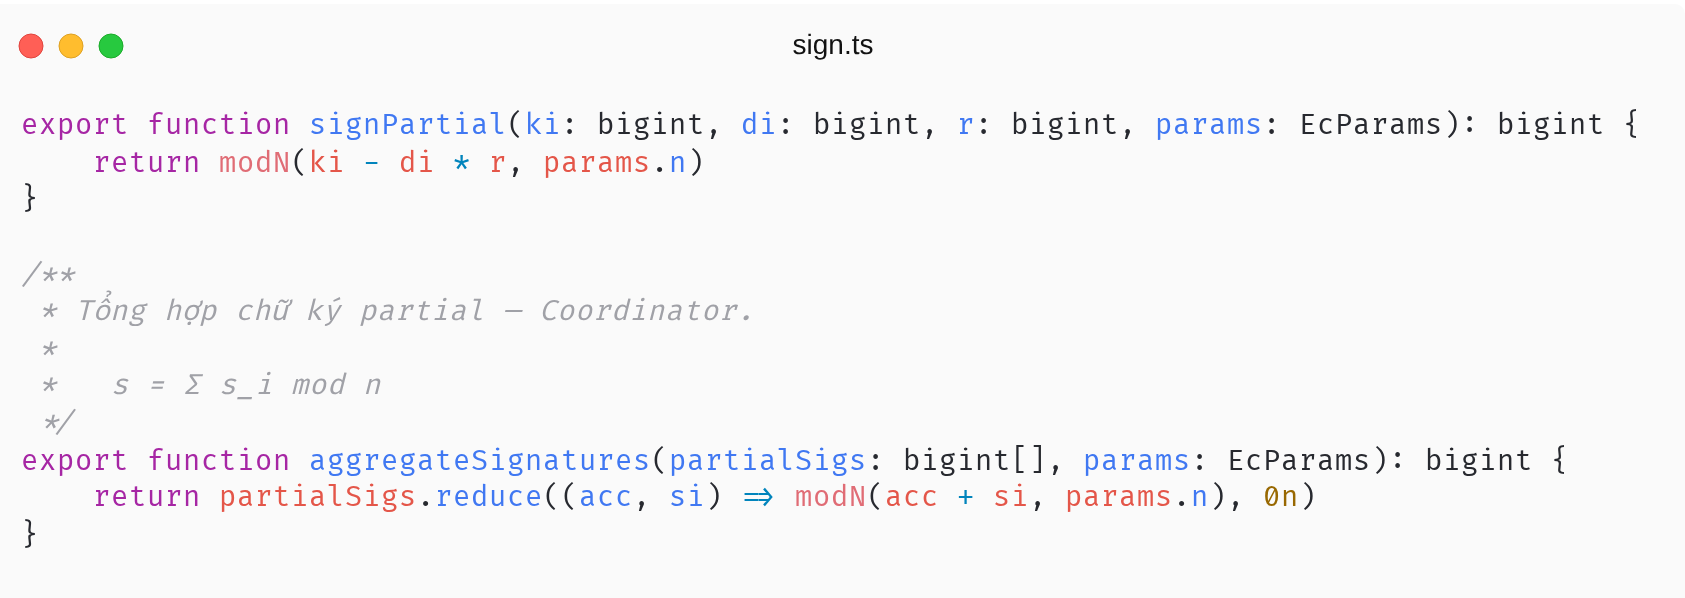
\includegraphics[width=0.9\textwidth, keepaspectratio]{Figures/code/ec-schnorr-sign.png}
    \caption{Hàm \pkg{signPartial} và \pkg{aggregateSignatures} trong thư viện \pkg{ec-schnorr}}
    \label{fig:ec-schnorr-sign}
\end{figure}

\subsubsection{Tính chất bảo mật được đảm bảo}

Lược đồ ký mù tập thể EC-Schnorr triển khai trong hệ thống cung cấp ba tính chất bảo mật cốt lõi:

\begin{itemize}
    \item \textbf{Tính mù (\textit{Blindness}):} máy chủ chỉ thấy giá trị \textit{thử thách đã làm mù} $r$ và \textit{cam kết đã làm mù} dưới dạng băm $\text{SHA256}(C')$. Không tồn tại cách thức tính toán hiệu quả để phục hồi \pkg{candidateId} hay cặp $(\alpha, \beta)$ từ các giá trị này.

    \item \textbf{Tính không liên kết (\textit{Unlinkability}):} do $r = (h - \beta) \bmod n$ phụ thuộc vào $\beta$ được sinh ngẫu nhiên ở mỗi lần bỏ phiếu, hai phiếu cùng nội dung cũng sinh ra hai giá trị $r$ khác nhau. Máy chủ không có khả năng liên kết một $r$ trong pha ký với một phiếu được công bố trong pha giải mù sau này.

    \item \textbf{Chống tấn công phát lại liên bầu cử (\textit{Cross-election replay prevention}):} thông điệp $M$ được gắn định danh bầu cử qua \textit{domain separator} \textit{``ev-vote-v1''} kết hợp \pkg{electionId}. Một chữ ký hợp lệ trong bầu cử $A$ khi xác thực trong bầu cử $B$ sẽ thu được $h_{check} \neq h$ vì thông điệp $M$ khác.
\end{itemize}

Toàn bộ thư viện \pkg{ec-schnorr} của hệ thống được hiện thực dựa trên \pkg{@noble/curves} (\pkg{secp256k1}) và \pkg{@noble/hashes} (SHA-256) — các thư viện cài đặt theo thời gian hằng (\textit{constant-time}), không phụ thuộc native binding và chạy được trên cả Node.js lẫn trình duyệt, qua đó cho phép cử tri tự kiểm chứng chữ ký bằng cùng một mã nguồn ngay tại máy của mình.
